
%-------------------------------------------------------------------------------
%							THIRD SECTION
%-------------------------------------------------------------------------------



\section{\textsc{Travaux et résultats 1D}}


\subsection{Déplacement des n\oe{}uds}

\begin{frame}{Déplacement des noeuds d’un floe isolé (1)}

    \mycols{

        \mycol{50}{
            \myfigframe{Deplacement1D-Systeme.png}{Floe de glace 1D}

            \begin{figure}[!h]
                \begin{subfigure}[b]{0.47\textwidth}
                    \centering
                    \frame{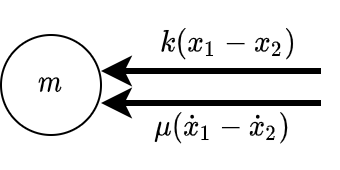
\includegraphics[width=\textwidth]{Deplacement1D-Masse1.png}}
                    % \caption{Sur la masse $m$ de gauche.}
                \end{subfigure}
                \begin{subfigure}[b]{0.43\textwidth}
                    \centering
                    \frame{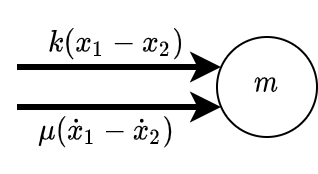
\includegraphics[width=\textwidth]{Deplacement1D-Masse2.png}}
                    % \caption{Sur la masse $m$ de droite.}
                \end{subfigure}
                   \caption{Bilan des forces}
            \end{figure}
        }

        \mycol{50}{
            Les équations de Newton-Euler:
            \begin{align*}
                \begin{dcases}
                m\ddot x_1 = - k(x_1 - x_2) - \mu(\dot x_1 - \dot x_2) \,,\\
                    m \ddot x_2 =  k(x_1 - x_2) + \mu(\dot x_1 - \dot x_2) \,. 
                \end{dcases}
            \end{align*}

            On préfère la forme matricielle:
            \begin{align*}
                \begin{dcases}
                    \dot{Y}(t)= E Y(t) \,,\\
                    Y_0 = Y(0) = (0,0,v_0,-v'_0)^T \,,
                \end{dcases}
            \end{align*}

            où :
            \begin{align*}
                E = \begin{pmatrix}
                    0 & 0 & 1 & 0 \\ 0 & 0& 0& 1 \\ -\frac{k}{m} & \frac{k}{m} & -\frac{\mu}{m} & \frac{\mu}{m} \\ \frac{k}{m} & -\frac{k}{m} & \frac{\mu}{m} & -\frac{\mu}{m}
                \end{pmatrix} \,,
                \text{ et } Y = \begin{pmatrix} x_1 \\ x_2 \\ \dot{x}_1 \\ \dot{x}_2 \end{pmatrix} 
            \end{align*}
        }
    }

    \note{Ici, ne pas utiliser un repère absolu, on peut utiliser un qui soit relatif au floe. Dans ce cas, on a convergence.}
    
\end{frame}


\begin{frame}[fragile]{Déplacement des noeuds d’un floe isolé (2)}

    \begin{columns}[onlytextwidth]
		
		\small
        \begin{column}{0.4\textwidth}
            \begin{lstlisting}[language=Python,captionpos=b,caption=Code de simulation]
    Y0 = np.array([0,0, v0, -v_0])
    t = np.linspace(0, tmax, N+1)
    def model(Y, t):
        return E @ Y
    Y = odeint(model, Y0, t)
            \end{lstlisting}
        \end{column}

		\normalsize
        \mycol{60}{    
        \begin{exampleblock}{Théorème (Convergence du modèle 1D isolé)}
            Partant d'une position d'équilibre $x_1(0) = x_2(0) = 0$, les déplacements $x_1(\cdot)$ et $x_2(\cdot)$ des deux n\oe{}uds du floe 1D (avec viscosité $\mu > 0$) convergent  si et seulement si leurs vitesses initiales sont opposées, i.e. $\bvec v_0 = - \bvec v'_0$.
        \end{exampleblock}
        }
    \end{columns}
    

    
    \begin{figure}[!h]
        \centering
        \begin{subfigure}[t]{0.45\textwidth}
            \centering
            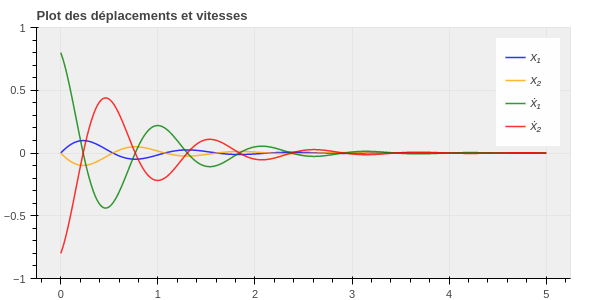
\includegraphics[width=\textwidth]{SimuDeplacement1D1.png}
            \caption{$v_0=v'_0 = 0.8$}
        \end{subfigure}
        \begin{subfigure}[t]{0.45\textwidth}
            \centering
            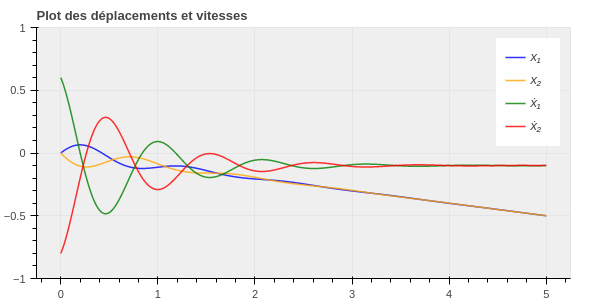
\includegraphics[width=\textwidth]{SimuDeplacement1D2.png}
            \caption{$v_0= 0.6$ et $v'_0 = 0.8$}
        \end{subfigure}    
        \caption{Simulation du déplacement d'un floe 1D à 2 n\oe{}uds}
    \end{figure}

\end{frame}





\subsection{Percussion entre floes}



\begin{frame}{Collision parfaitement inélastique avec un floe encastré}

    \mycols{

        \mycol{55}{
            \myfigframe{Percussion1D-Systeme}{Collision 1D avec fixation d'un floe}

            \begin{figure}[!h]
                \begin{subfigure}[b]{0.54\textwidth}
                    \centering
                    \frame{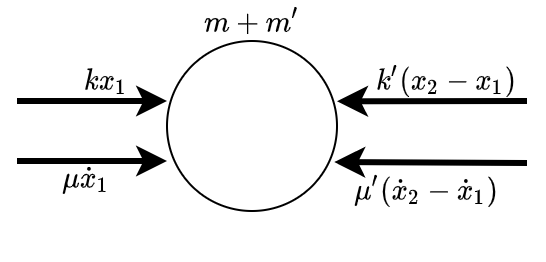
\includegraphics[width=\textwidth]{Percussion1D-Masse1}}
                \end{subfigure}
                \begin{subfigure}[b]{0.435\textwidth}
                    \centering
                    \frame{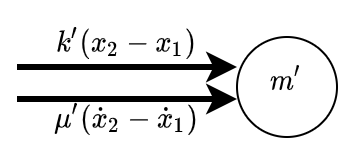
\includegraphics[width=\textwidth]{Percussion1D-Masse2}}
                \end{subfigure}
                   \caption{Bilan des forces}
            \end{figure}

            Le système est régi par les équations :
            \begin{align*}
                \begin{dcases}
                (m+m')\ddot x_1 = -kx_1 - \mu \dot x_1 + k'(x_2 - x_1) + \mu'(\dot x_2 - \dot x_1) \,, \\
                    m' \ddot x_2 =  -k'(x_2 - x_1) - \mu'(\dot x_2 - \dot x_1). 
                \end{dcases}
            \end{align*}

        }

        \mycol{45}{

            \myfig{SimuPercussion1D.png}{Résultat de simulation}
        }

    }
    
\end{frame}


\begin{frame}{Collision parfaitement inélastique sans présence du mur}

    \mycols{

        \mycol{55}{
            \myfigframe{Percussion1D-Systeme-2}{Collision 1D sans mur}

            \begin{figure}[!h]
                \begin{subfigure}[b]{0.30\textwidth}
                    \centering
                    \frame{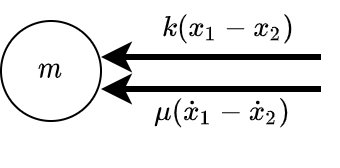
\includegraphics[width=\textwidth]{Percussion1D2-Masse1.png}}
                \end{subfigure}
                \begin{subfigure}[b]{0.38\textwidth}
                    \centering
                    \frame{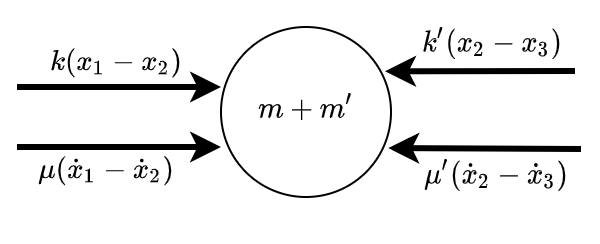
\includegraphics[width=\textwidth]{Percussion1D2-Masse2}}
                \end{subfigure}
                \begin{subfigure}[b]{0.26\textwidth}
                    \centering
                    \frame{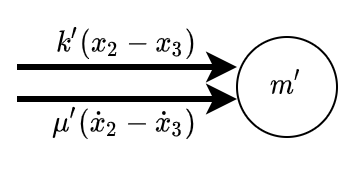
\includegraphics[width=\textwidth]{Percussion1D2-Masse3}}
                \end{subfigure}
                   \caption{Bilan des forces}
            \end{figure}

            Le système est régi par les équations :
            \begin{align*}
                \begin{dcases}
                m\ddot x_1 = -k(x_1 - x_2) - \mu (\dot x_1 - \dot x_2) \,, \\
                (m+m')\ddot x_2 = k(x_1 - x_2) + \mu (\dot x_1 - \dot x_2) - k'(x_2 - x_3) - \mu'(\dot x_2 - \dot x_3) \,, \\
                    m' \ddot x_3 =  k'(x_2 - x_3) + \mu'(\dot x_2 - \dot x_3) \,. 
                \end{dcases}
            \end{align*}

        }

        \mycol{45}{
            % \myfig{SimuPercussion1D2.png}{Résultat de simulation}

            \vspace*{-0.25cm}

            \begin{figure}[!h]
                \begin{subfigure}[t]{\textwidth}
                    \centering
                    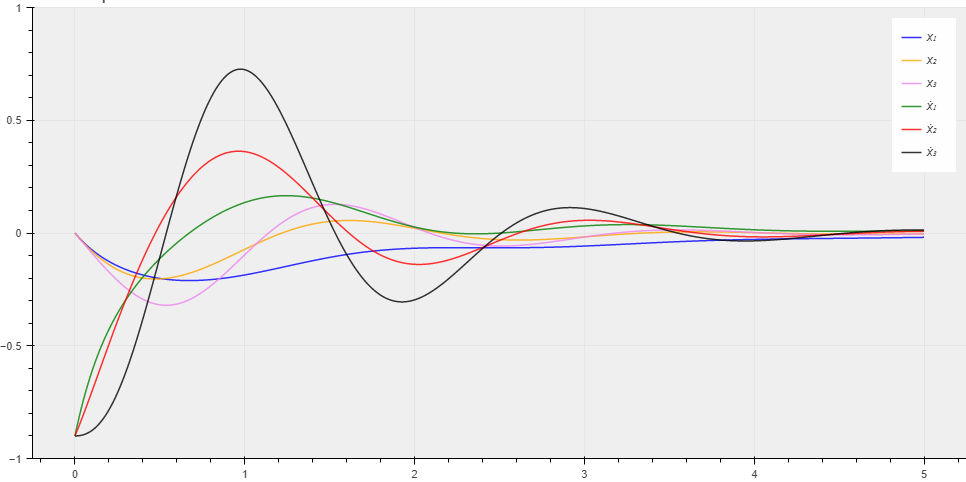
\includegraphics[width=0.9\textwidth]{SimuPercussion1D2.png}
                    \caption{Cas convergent}
                \end{subfigure}
                \begin{subfigure}[t]{\textwidth}
                    \centering
                    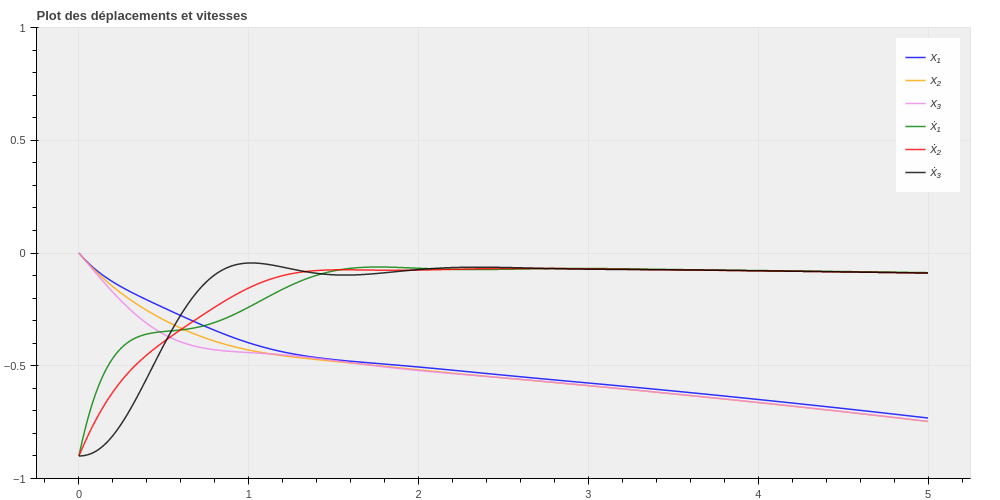
\includegraphics[width=0.9\textwidth]{SimuPercussion1D2NonConv.png}
                    \caption{Cas non convergent}
                \end{subfigure}
                   \caption{Résultats de simulation}
            \end{figure}

			\scriptsize
            \begin{alertblock}{Note}
                Le critère de convergence n'est pas clair (i.e. $\mu << \mu'$, etc.)!
            \end{alertblock}
            \normalsize

        }

    }
    
\end{frame}


\begin{frame}{Collision inélastique avec séparation des masses}

    \mycols{

        \mycol{50}{
            \myfigframe{Percussion1D-Systeme-3}{Collision 1D inélastique}

            \vspace*{-0.5cm}
            \begin{figure}[!h]
                \begin{subfigure}[b]{0.35\textwidth}
                    \centering
                    \frame{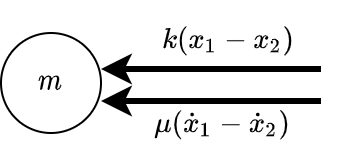
\includegraphics[width=\textwidth]{Percussion1D3-Masse1.png}}
                \end{subfigure}
            %     \hfill
                \begin{subfigure}[b]{0.48\textwidth}
                    \centering
                    \frame{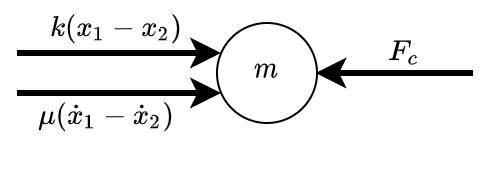
\includegraphics[width=\textwidth]{Percussion1D3-Masse2}}
                \end{subfigure}
            %     \hfill
                \begin{subfigure}[b]{0.44\textwidth}
                    \centering
                    \frame{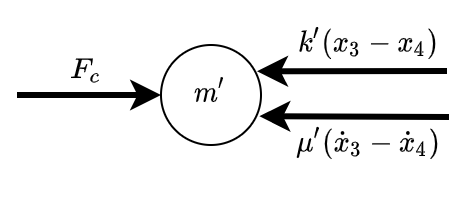
\includegraphics[width=\textwidth]{Percussion1D3-Masse3}}
                \end{subfigure}
            %     \hfill
                \begin{subfigure}[b]{0.35\textwidth}
                    \centering
                    \frame{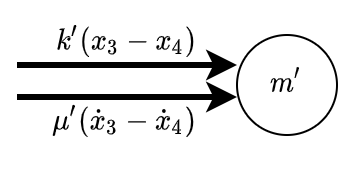
\includegraphics[width=\textwidth]{Percussion1D3-Masse4}}
                \end{subfigure}
                   \caption{Bilan des forces}
            \end{figure}

            \vspace*{-0.5cm}
            \myfigframe{Percussion1D3-Apres.png}{Situation \alert{après} contact}

        }

        \mycol{50}{
            Le système est régi par les équations :
            \begin{align*}
                \begin{dcases}
                m\ddot x_1 = -k(x_1 - x_2) - \mu (\dot x_1 - \dot x_2) \,, \\
                m\ddot x_2 = k(x_1 - x_2) + \mu (\dot x_1 - \dot x_2) - \alert{F_c} \,, \\
                m'\ddot x_3 = - k'(x_3 - x_4) - \mu'(\dot x_3 - \dot x_4) + \alert{F_c} \,, \\
                    m' \ddot x_4 =  k'(x_3 - x_4) + \mu'(\dot x_3 - \dot x_4) \,. 
                \end{dcases}
            \end{align*}

            Avec $\varepsilon$ est le coefficient de restitution et :
            \scriptsize
            $$
            I = \int_{\tmoins}^{\tplus} k(x_1 - x_2) + \mu (\dot x_1 - \dot x_2) - k'(x_3 - x_4) - \mu'(\dot x_3 - \dot x_4) \diff t \,,
            $$
            \normalsize
            les vitesses après contact sont :
            \begin{align*}
                V_0 = \frac{I + (m-\varepsilon m')v_0 + (1+\varepsilon)m'v'_0}{m+m'}\,, \\
                V'_0 = \frac{I + (1+\varepsilon)mv_0 + (m'-\varepsilon m)v'_0}{m+m'}\,.
            \end{align*}
            
            \note{Le calcul des vitesses ici était notre première tentative de trouver ce qui se passe véritablement après un contact. Nous avons complexifier les choses par la suite.}

        }

    }
    
\end{frame}




\begin{frame}{Des modèles généraux pour la percussion avec séparation des masses (1)}

	\myfigframesize{Deplacement1D-2.png}{Illustration d'un floe 1D contenant $n$ masses}{80}
	
	\small
	\vspace*{-0.1cm}
	Sous forme matricielle, on a le système:
	\begin{align} \label{eq:percussion1d4}
    \begin{pmatrix}
        \dot z_0 \\ \dot z_1 \\ \vdots \\ \dot z_{n-1} \\ \ddot z_0 \\ \ddot z_1 \\ \vdots \\ \ddot z_{n-1}
    \end{pmatrix}
    = 
    \underbrace{\begin{pmatrix}
        \begin{matrix}
       & & &  \\ & & &  \\ & & \bigzero & \\ & & & \\      
        \end{matrix}
        & \rvline 
        & \begin{matrix}
        & & & \\ & & &  \\ & & I_n & \\ & & & \\
        \end{matrix}  \\ 
        \hline
        \begin{matrix}
            & & &  \\ & & B & \\ & & & \\ & & & \\     
        \end{matrix}
        & \rvline 
        &\begin{matrix}
            & & & \\ & & C & \\ & & & \\ & & & \\        
        \end{matrix}
      \end{pmatrix}}_{2n \times 2n}
      \begin{pmatrix}
        z_0 \\ z_1 \\ \vdots \\ z_{n-1} \\ \dot z_0 \\ \dot z_1 \\ \vdots \\ \dot z_{n-1}
        \end{pmatrix}
    +
    \underbrace{\begin{pmatrix}
        \begin{matrix}
       & & &  \\ & & &  \\ & & \bigzero & \\ & & & \\      
        \end{matrix}
        & \rvline 
        &     \begin{matrix}
            & & &  \\ & & &  \\ & & \bigzero & \\ & & & \\      
             \end{matrix}  \\ 
        \hline
        \begin{matrix}
            & & &  \\ & & D & \\ & & & \\ & & & \\     
        \end{matrix}
        & \rvline 
        &   \begin{matrix}
            & & &  \\ & & \bigzero &  \\ & &  & \\ & & & \\      
            \end{matrix}
      \end{pmatrix}}_{(2n) \times (2n-2)}
      \begin{pmatrix}
        L0_0 \\ L0_1 \\ \vdots \\ L0_{n-2} \\ 0 \\ 0 \\ \vdots \\ 0
        \end{pmatrix} \,,
	\end{align}
	
	où:
	\scriptsize
	$$
B = \frac{1}{m} \begin{pmatrix}
    -k & k &  &  &  \\
    k & -2k & k &  &  \\
     & \ddots & \ddots & \ddots &  \\
     &  & k & -2k & k \\
     &  &  & k & -k
    \end{pmatrix} , 
C = \frac{1}{m} \begin{pmatrix}
    -\mu & \mu &  &  &  \\
    \mu & -2\mu & \mu &  &  \\
     & \ddots & \ddots & \ddots &  \\
     &  & \mu & -2\mu & \mu \\
     &  &  & \mu & -\mu
    \end{pmatrix} , 
D = \frac{1}{m} \begin{pmatrix}
    -k &  &  &  \\
    k & -k &  &  \\
     & \ddots & \ddots &  \\
     &  & \ddots & -k \\
     &  &  & k 
    \end{pmatrix}.
	$$
    \normalsize
\end{frame}


\begin{frame}{Des modèles généraux pour la percussion avec séparation des masses (2)}

\begin{figure}[!h]
    \begin{subfigure}[b]{0.30\textwidth}
        \centering
        \frame{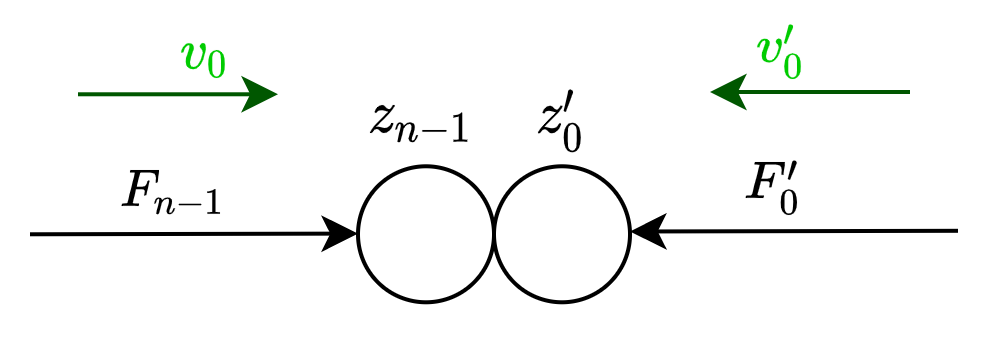
\includegraphics[width=\textwidth]{Percussion1D-4-Avant.png}}
        \caption{Avant le choc}
    \end{subfigure}
%     \hfill
    \begin{subfigure}[b]{0.29\textwidth}
        \centering
        \frame{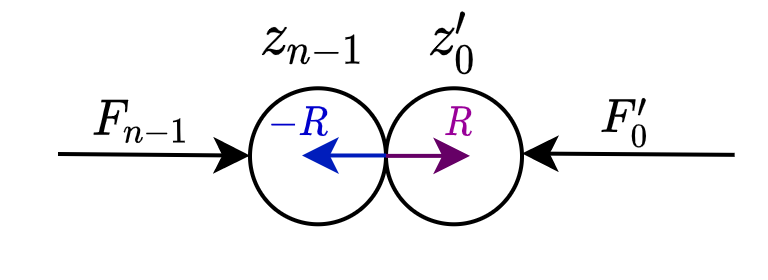
\includegraphics[width=\textwidth]{Percussion1D-5.png}}
        \caption{Pendant le choc}
    \end{subfigure}
    \begin{subfigure}[b]{0.30\textwidth}
        \centering
        \frame{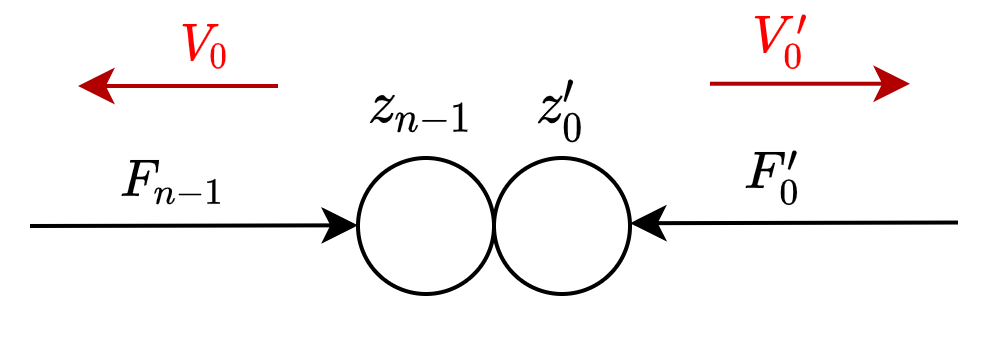
\includegraphics[width=\textwidth]{Percussion1D-4-Apres.png}}
        \caption{Après le choc}
    \end{subfigure}
\end{figure}


%\myfigframesize{Percussion1D-4-Avant.png}{Avant le choc}{40}
%\myfigframesize{Percussion1D-4-Apres.png}{Après le choc}{40}


	\mycols{
		\mycol{50}{	
        \begin{alertblock}{Un modèle qui conserve l'énergie cinétique après chaque choc.}
        \begin{align}
			V_0 = \frac{-b \pm \sqrt{\Delta}}{2a}, \quad V'_0 = V_0 + X\,,
		\end{align}
		avec :
		\begin{align*}
		X = \varepsilon(v_0 - v'_0)&, \, Y = m(v_0)^2 + m'(v'_0)^2\,,\\  a &= m+m'\,,\\ b &= -2m'X\,,\\ c &= m'X^2 - Y \,,\\ \Delta &= b^2 - 4ac.
		\end{align*}
		\end{alertblock}
		}
		
		\mycol{50}{	
        \begin{exampleblock}{Un modèle qui met en évidence le coefficient de restitution \parencite{hecker1997collision}.}
		\begin{align} \label{eq:perc5eq2}
    V_0 = v_0 + \frac{J-I}{m} , \quad
    V'_0 = v'_0 + \frac{K+I}{m'}\,,
		\end{align}
		avec:
		\begin{align*}
    I = \frac{(v_0 - v'_0)(1+\varepsilon) +\frac{J}{m} - \frac{K}{m'}}{\frac{1}{m}+\frac{1}{m'}}, \\
    		J = \int_{t^{-}}^{t^{+}} F_{n-1} \diff t = F_{n-1} \, \Delta t, \\ 
    		K = \int_{t^{-}}^{t^{+}} F'_{0} \diff t = F'_{0} \, \Delta t.
		\end{align*}

		\end{exampleblock}
		}
		
		\note{Technique répandue dans le monde du jeux vidéo pour le codage des graphics engines!!}

	}
\end{frame}



\begin{frame}{Des modèles généraux pour la percussion avec séparation des masses (3)}

	\myfig{Screenshot1.jpg}{Configuration des floes pour la simulation}

	\mycols{
		\mycol{50}{	
        \begin{alertblock}{\vspace*{-0.5cm}}
		\myfig{EnsPlotPerc2.png}{Résultat pour le modèle qui conserve l'énergie cinétique après chaque choc}
		\vspace*{-0.4cm}
		\end{alertblock}
		}
		
		\mycol{50}{	
        \begin{exampleblock}{\vspace*{-0.5cm}}
		\myfig{EnsPlotPerc3.png}{Résultat pour le modèle qui met en évidence le coefficient de restitution}
		\vspace*{-0.4cm}
		\end{exampleblock}
		}
		
		\note{Technique répandue dans le monde du jeux vidéo pour le codage des graphics engines!!}

	}
\end{frame}









\subsection{Fracturation des floes}


\begin{frame}{Différents modèles de fracture fragile}

\vspace{-0.5cm}
\myfigsize{PhaseFieldExplainer.png}{Champ de phase pour la régularisation d'une fissure \parencite{yvonnet2018fissuration}}{45}
\vspace{-0.5cm}
	
	\mycols{
		\mycol{45}{	
        \begin{block}{Méthode du champ de phase}
        \vspace{-0.4cm}
        \small
\begin{align*}
    E = \int_{\Omega} \Psi(\bvec{u},\Gamma) &\diff\Omega + G_c\int_{\Gamma} \diff \Gamma, \\
&\big\Downarrow \\
    E = \int_{\Omega} \Psi(\bvec{u},\Gamma) \diff\Omega &+ G_c\int_{\Gamma} \textcolor{orange}{\gamma(d, \nabla d)} \diff \Gamma.
\end{align*}
		 \vspace{-0.2cm} 
		\end{block}
		}

		\normalsize
		\mycol{55}{	
        \begin{block}{Méthode combinatoire}
            \begin{align*} \label{eq:modelcombi}
                E^{n+1} & = \text{eng. pot. élastique au temps } t^{n+1}  \\
                & + \text{ ténacité}\times \text{lg. de la fracture envisagée à }t^{n+1}.  
            \end{align*}
		\vspace*{0.001cm} 
		\end{block}
		}

	}
	\vspace{0.2cm}


	\centering
    \textcolor{mygray}{\href{run:../../../../Share/ShortAnim2D.gif}{\textbf{Animation de la fracture 1D par un algorithme \emph{event-driven}}}}

	\animategraphics[loop,controls,autoplay,width=\linewidth]{10}{Simu1D/FracSimu-}{0}{312}
	
\end{frame}




